\documentclass[10pt,a4paper]{article}
\renewcommand{\familydefault}{\sfdefault}
\usepackage{svg}
\usepackage{amssymb}
\usepackage{multicol}
\usepackage{listings}
\usepackage{color}
\usepackage{mdframed}

\renewcommand{\land}{\,\&\,}

\definecolor{dkgreen}{rgb}{0,0.6,0}
\definecolor{gray}{rgb}{0.5,0.5,0.5}
\definecolor{mauve}{rgb}{0.58,0,0.82}

\usepackage{amsmath}
\usepackage{graphicx}
\usepackage{tikz}
\usepackage{amssymb}
\usepackage[skip=10pt plus1pt, indent=0em]{parskip}
\usepackage{titlesec}

\usepackage{setspace}

\usepackage[margin=1in]{geometry}

\author{Aaron Po}

\begin{document}

\title{Notes on Collision Detection and Collision Resolution}
\date{July 2024}
% \maketitle

\section{Introduction}
This document contains notes on collision detection and collision resolution.
These notes are based on course material from COMP 4300 at the Memorial
University of Newfoundland taught by Prof.\ David Churchill.

\section{Collision Detection}
\subsection{Collision Detection Problems}
\begin{itemize}
    \item Given two entities which have a current position, do they intersect?
          \begin{enumerate}
              \item If they do intersect, how do we resolve the collision?
              \item If they do not intersect, how do we determine if they will intersect in the
                    future?
          \end{enumerate}

          \begin{figure}[ht]
              \centering

              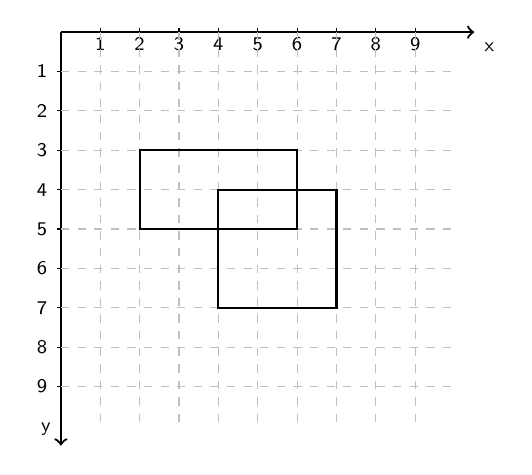
\begin{tikzpicture}
                  % Transform the canvas so (0,0) is at the top left and scale it down by half
                  \begin{scope}[yscale=-1, yshift=-5cm, scale=0.5]
                      % Draw x and y axes with arrows
                      \draw[thick,->] (0,0) -- (10.5  ,0) node[anchor=north west] {\scriptsize x};
                      \draw[thick,->] (0,0) -- (0,10.5) node[anchor=south east] {\scriptsize y};

                      % Draw x-axis tick marks and labels
                      \foreach \x in {1,2,...,9}
                      \draw (\x,0.1) -- (\x,-0.1) node[anchor=north] {\scriptsize \x};

                      % Draw y-axis tick marks and labels
                      \foreach \y in {1,2,...,9}
                      \draw (0.1,\y) -- (-0.1,\y) node[anchor=east] {\scriptsize \y};

                      % Draw light gray grid lines
                      \foreach \x in {1,2,...,9}
                      \draw[lightgray,dashed] (\x,0) -- (\x,10);
                      \foreach \y in {1,2,...,9}
                      \draw[lightgray,dashed] (0,\y) -- (10,\y);

                      % Draw the first non-colored non-square box
                      \draw[thick] (2,3) rectangle (6,5);
                      % Draw the second non-colored non-square box
                      \draw[thick] (4,4) rectangle (7,7);
                  \end{scope}
              \end{tikzpicture}

              \caption{Intersecting Boxes}
              \label{fig:intersecting_boxes}
          \end{figure}
\end{itemize}

\subsection{Entity Bounding Shapes}
Everyday objects have arbitrary shapes and interaction surfaces. For example,
consider a teacup. A teacup has a complex shape consisting of many curves and
edges. Accurately simulating the collision of a teacup requires considering
both the teacup's shape and the shape of the object it collides with. With many
complex shapes, collision detection becomes computationally expensive.

To address this issue, we use bounding shapes that approximate an object's
shape to calculate collisions more efficiently. The most effective way to do
this is by using primitive types:

\begin{itemize}
    \item \textbf{2D:} Circle, Rectangle, Triangle, Octagon
    \item \textbf{3D:} Sphere, Box, Cylinder, Cone
\end{itemize}

The circle is a common primitive shape and is the simplest possible
intersection bounding shape. Another commonly used shape is the rectangle,
which encloses an object in a box.

By using these primitive shapes, collision detection becomes simpler and less
computationally demanding.

\subsubsection{Bounding Circles}
As mentioned, the circle is the simplest possible intersection bounding shape
in regards to collision detection. This is because a circle is only defined
only by its center and radius, making calculations for collision detection
easier.

Calculating the distance between two circles is a simple task. Given two
circles with centers $c_1$ and $c_2$ and radii $r_1$ and $r_2$, the distance
between the two circles is given by the formula:

\begin{equation}
    d = \sqrt{(c_2.x - c_1.x)^2 + (c_2.y - c_1.y)^2}
\end{equation}

This is derived from the Pythagorean theorem, where the length of the
hypotenuse of a right triangle is given by the square root of the sum of the
squares of the other two sides.

\begin{equation}
    c = \sqrt{a^2 + b^2}
\end{equation}

If the distance between the two circles is less than the sum of their radii,
then the circles intersect.

\begin{mdframed}
    \vspace{1em}

    \begin{lstlisting}[language=C++, aboveskip=3mm,
        belowskip=3mm,
        showstringspaces=false,
        columns=flexible,
        basicstyle={\small\ttfamily},
        numbers=left,
        numberstyle=\tiny\color{gray},
        keywordstyle=\color{blue},
        commentstyle=\color{dkgreen},
        stringstyle=\color{mauve},
        breaklines=true,
        breakatwhitespace=true,
        tabsize=3,
        xleftmargin=1em]
#include "Vec2.h"
#include <cmath>
#include <iostream>

struct Circle {
    Vec2 center;
    float radius;
};

bool checkCollision(const Circle &c1, const Circle &c2) {
    const float dx = c2.center.x - c1.center.x;
    const float dy = c2.center.y - c1.center.y;
    const float distance = std::sqrt(dx * dx + dy * dy);
    const float sumOfRadii = c1.radius + c2.radius;
    const bool collision = distance < sumOfRadii;

    return collision;
}
\end{lstlisting}

\end{mdframed}

\begin{center}
    \textbf{Listing 1:} \textit{Collision Detection for Bounding Circles in C++}
\end{center}

\subsubsection{Bounding Boxes}
In 2D games, objects are often enclosed in rectangles known as bounding boxes.
These are usually the smallest possible rectangle that completely encompasses
the texture's width and height. However, this is not always the case, as some
imperfections may exist such as the entity being larger than the bounding box.

Rectangles can be oriented in any direction as long as all four sides meet at
90-degree angles. This creates complexity in collision detection, requiring
calculations for line-line intersections. To simplify this, we can use
something called an axis-aligned bounding box (AABB). An AABB is a rectangle
that is aligned with the x and y axes, i.e. with sides parallel to the
coordinate axes.

The simplest calculation for AABBs is to check whether a point is inside the
rectangle. Given a point $p$ and a rectangle with corners $c_1$ and $c_2$, we
can determine if the point is inside the rectangle by checking if the point's x
and y coordinates are within the rectangle's x and y coordinates.

This is done by the following formula:

\begin{equation}
    \begin{aligned}
         & \textit{Point $P$ is inside rectangle with corners $c_1$ and $c_2$ if and only if:} \\
         & (p.x > c_1.x) \land (p.x < c_2.x) \land (p.y > c_1.y) \land (p.y < c_2.y)
    \end{aligned}
\end{equation}

broken down, the formula is evaluating four conditions:
\begin{multicols}{2}
    \begin{enumerate}
        \item The point's x-coordinate is to the right of the left side of the rectangle.
              \begin{equation}
                  p.x > c_1.x
              \end{equation}

        \item The point's x-coordinate is to the left of the right side of the rectangle.
              \begin{equation}
                  p.x < c_2.x
              \end{equation}

        \item The point's y-coordinate is above the bottom side of the rectangle.
              \begin{equation}
                  p.y > c_1.y
              \end{equation}

        \item The point's y-coordinate is below the top side of the rectangle.
              \begin{equation}
                  p.y < c_2.y
              \end{equation}
    \end{enumerate}
\end{multicols}

\end{document}
